\newpage
\section{Praktisk verkemåte}
\thispagestyle{fancy}

Sande reinseanlegg består av ``primærreinsing'' via grovrist, ein mottakstank 
som samlar varierande tilstrøymingar for å gi resten av anlegget homogene forhold og
``sekundær'' og ``tærtierreinsing'' ved to reaktorar som anvender \gls{SBR}-teknologi.

Avlaupsvatn vil opphalde seg i eller på veg mot ein av desse fire hovuddelane medan det er i anlegget.
Ferdig behandla avlaupsvatn blir drenert ut til resipient (elva Gaula). 

\begin{figure}[htbp]
    \centering
    \includegraphics[width=1\textwidth]{Figurar/Sande verkemåte.png} %% FIKS FIGUR
    \caption{\gls{RA}200 flytskjema}\label{fig:SandeVerkemaate}
\end{figure}


\subsection{Grovrist}
Innløpet på anlegget renn først gjennom grovrista. Grovrista på reinseanlegget
er ein ``HUBER ROTAMAT Ro9'' som er ei grovrist som nyttar ein mekanisk skrue.
Den fungerer som ein liten tank og ein intern nivågivar startar
skruen ved innkommande avlaupsvatn. Skruen tek med uorganisk materiale og fjernar det til eigen avfallshandtering.
Dersom grovrista er ute av drift vil vatn renne vidare til mottakstanken via eit overløpsrøyr.

\begin{figure}[htbp]
    \centering
    \begin{subfigure}[b]{0.3\textwidth}
        \centering
        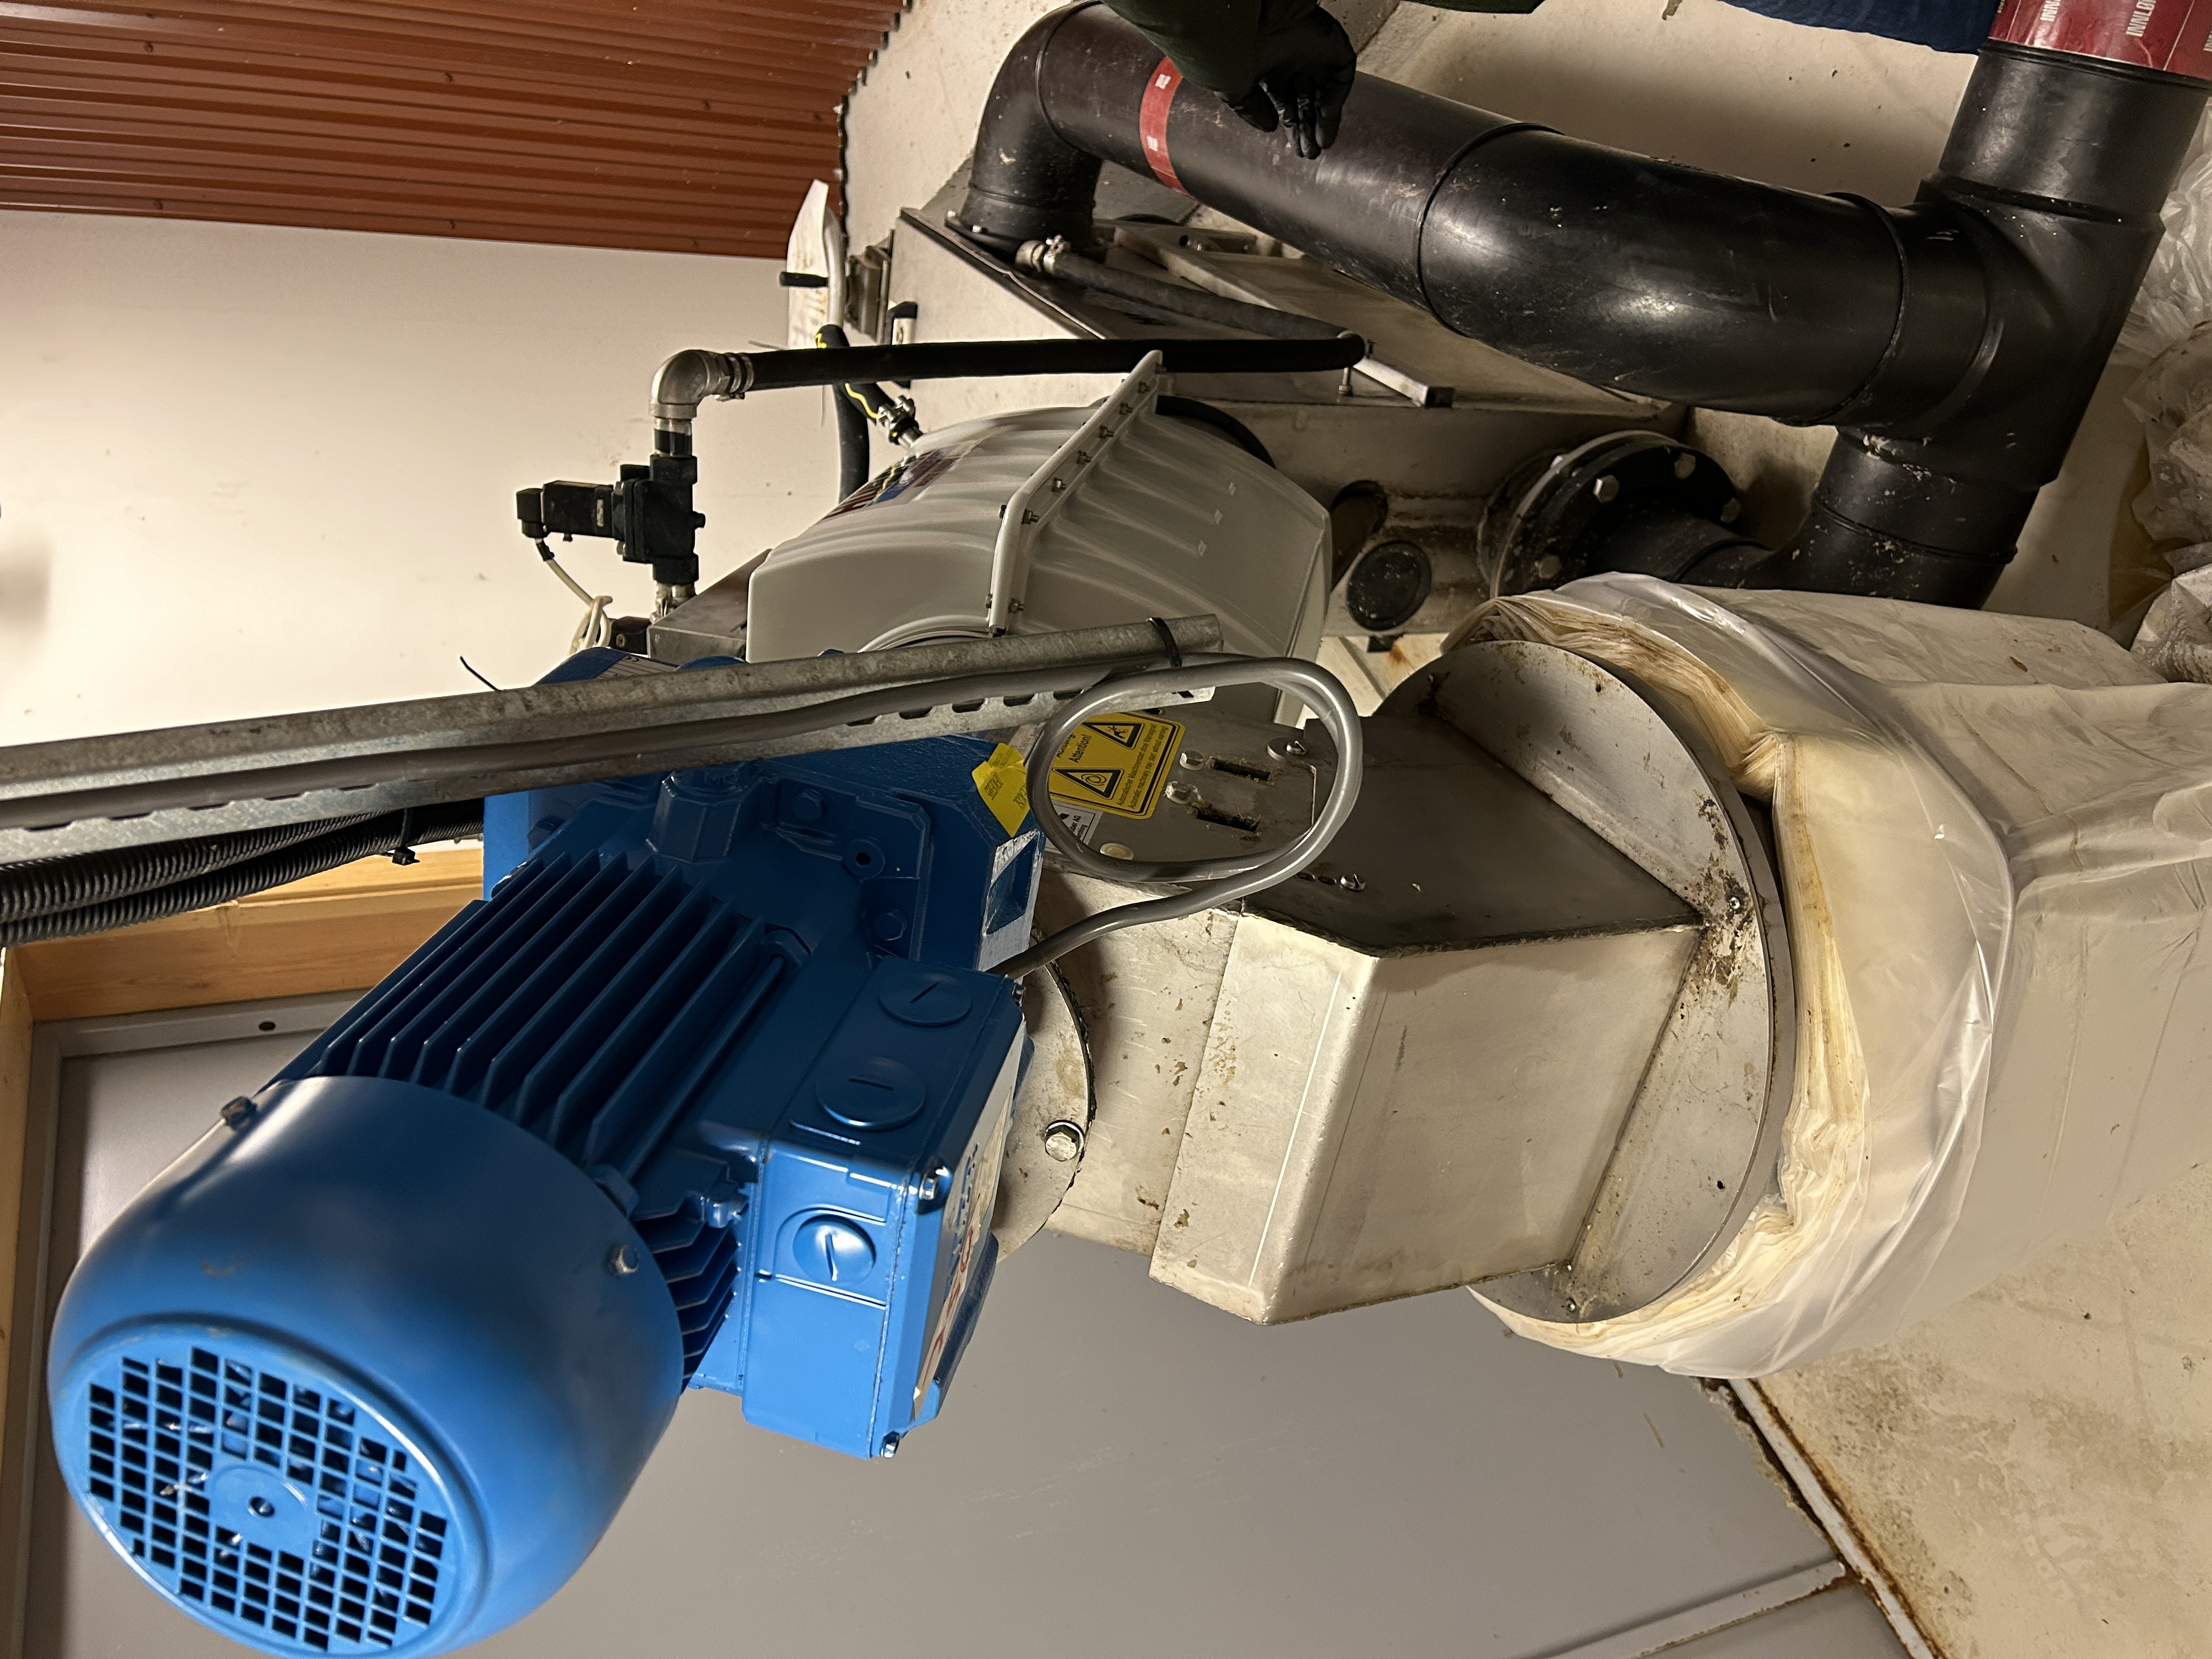
\includegraphics[angle=-90,width=1\textwidth]{Bilder/Huber.JPG}
        \caption{Motor og avfallshandtering}\label{fig:Huber}
    \end{subfigure}
    \hfill
    \begin{subfigure}[b]{0.3\textwidth}
        \centering
        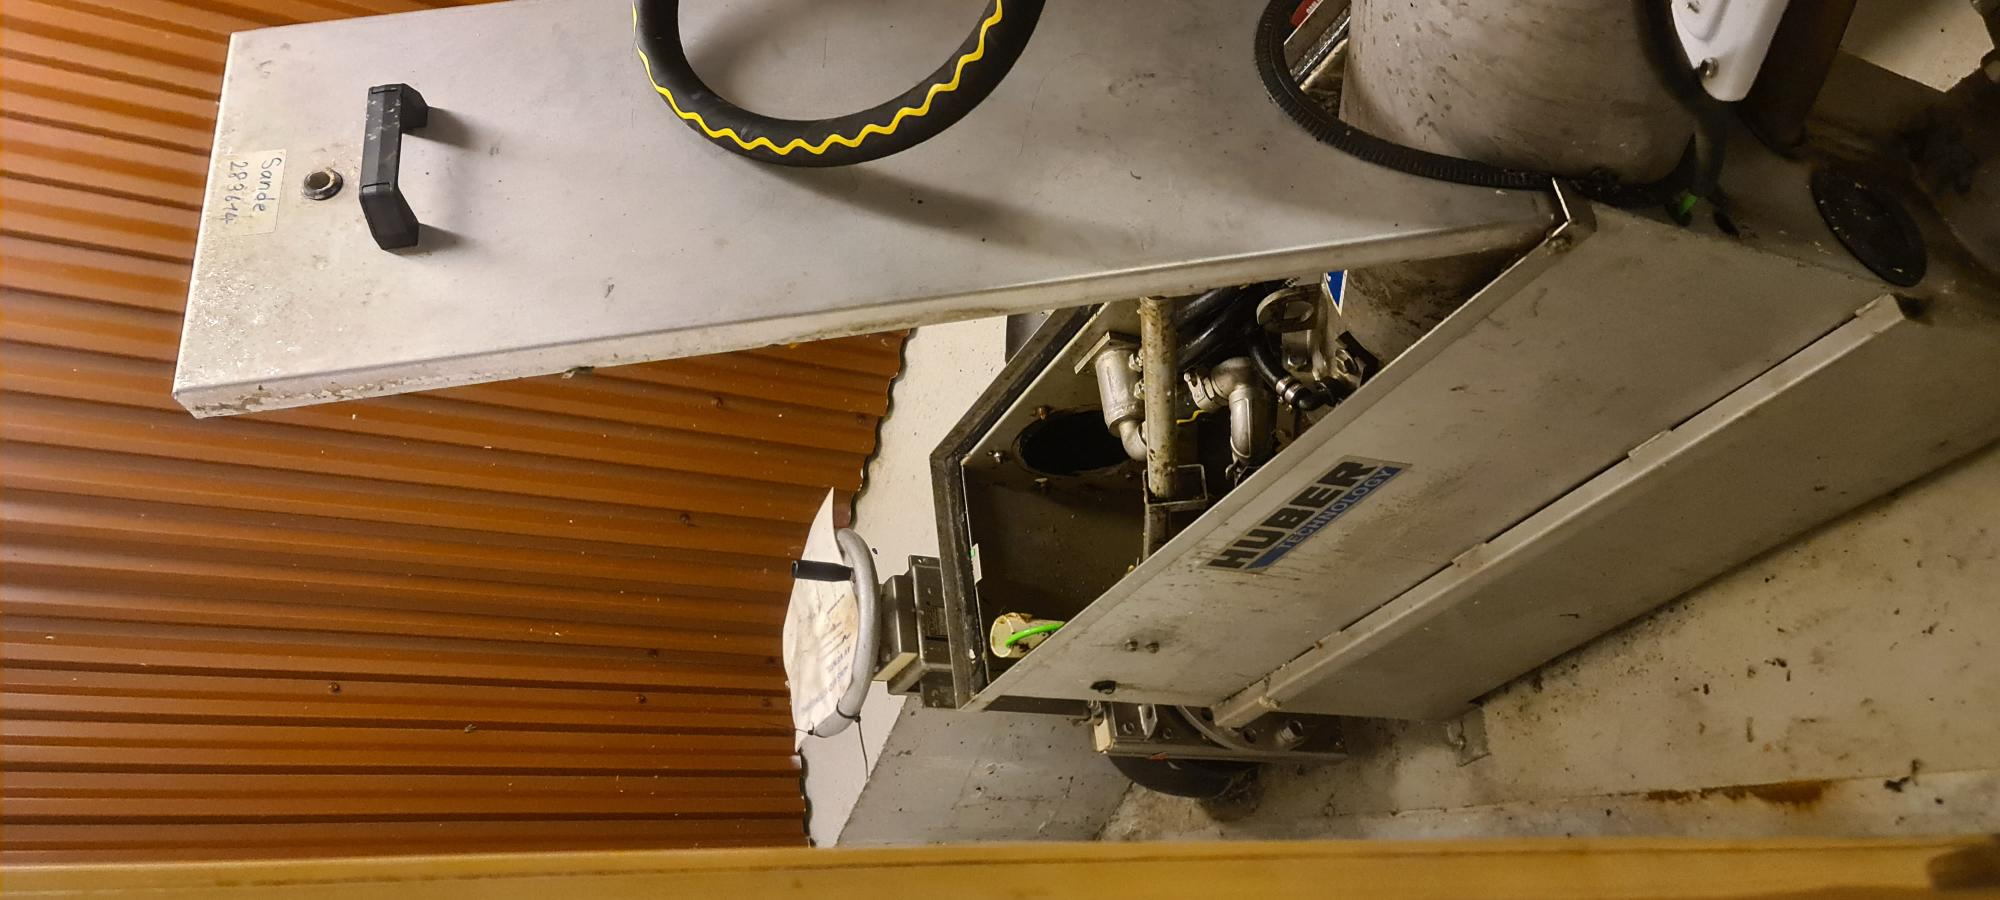
\includegraphics[angle=-90,width=0.6\textwidth]{Bilder/Huber2.JPG}
        \caption{Godts og skrue}\label{fig:Huber2}
    \end{subfigure}
    \caption{Grovrist levert av Huber}\label{fig:HuberGrovrist}
\end{figure}

\newpage
\subsection{Mottakstank}
Frå grovrista renn vatn med sjølvfall mot mottakstanken som ligg som lågaste punkt på anlegget.
Mottakstanken er 120 $m^3$ og er ein felles lagringsplass for vatn før det går vidare mot reaktorane.
Mottakstanken har fire sensorar som heng ifrå taket.

Nivået i mottakstanken blir primært målt med trykkgivar LT01. For at vatn skal pumpast vidare mot ein
reaktor i riktig sekvens må trykkgivar indikere at nivået er høgt nok. LS02 fungerar som backup. \newline
I toppen av mottakstanken er det ei overløpskasse som drenerer mot resipient, her vil det
ved normale omstendigheter ikkje renne anna ein reinsa vatn. Trykkgivar for overløp måler
dersom ureinsavatn renner i resipientrøyret.

%% Må endre på tegning fordi det eine navnet er feil. Ikkje reject frå sivbed.

\begin{figure}[htbp]
    \centering
    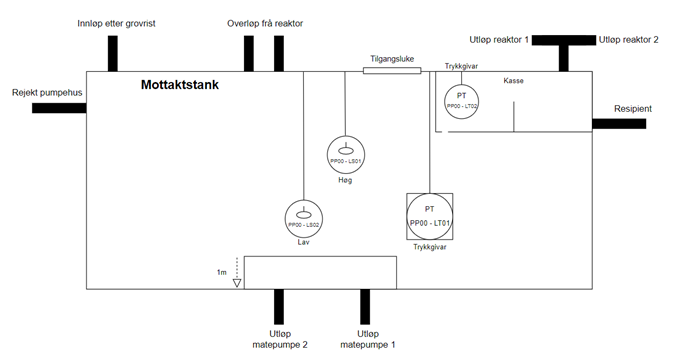
\includegraphics[width=1\textwidth]{Figurar/Mottakstank.png}
    \caption{P\&ID mottakstank}\label{fig:Mottakstank}
\end{figure}

\begin{figure}[htbp]
    \centering
    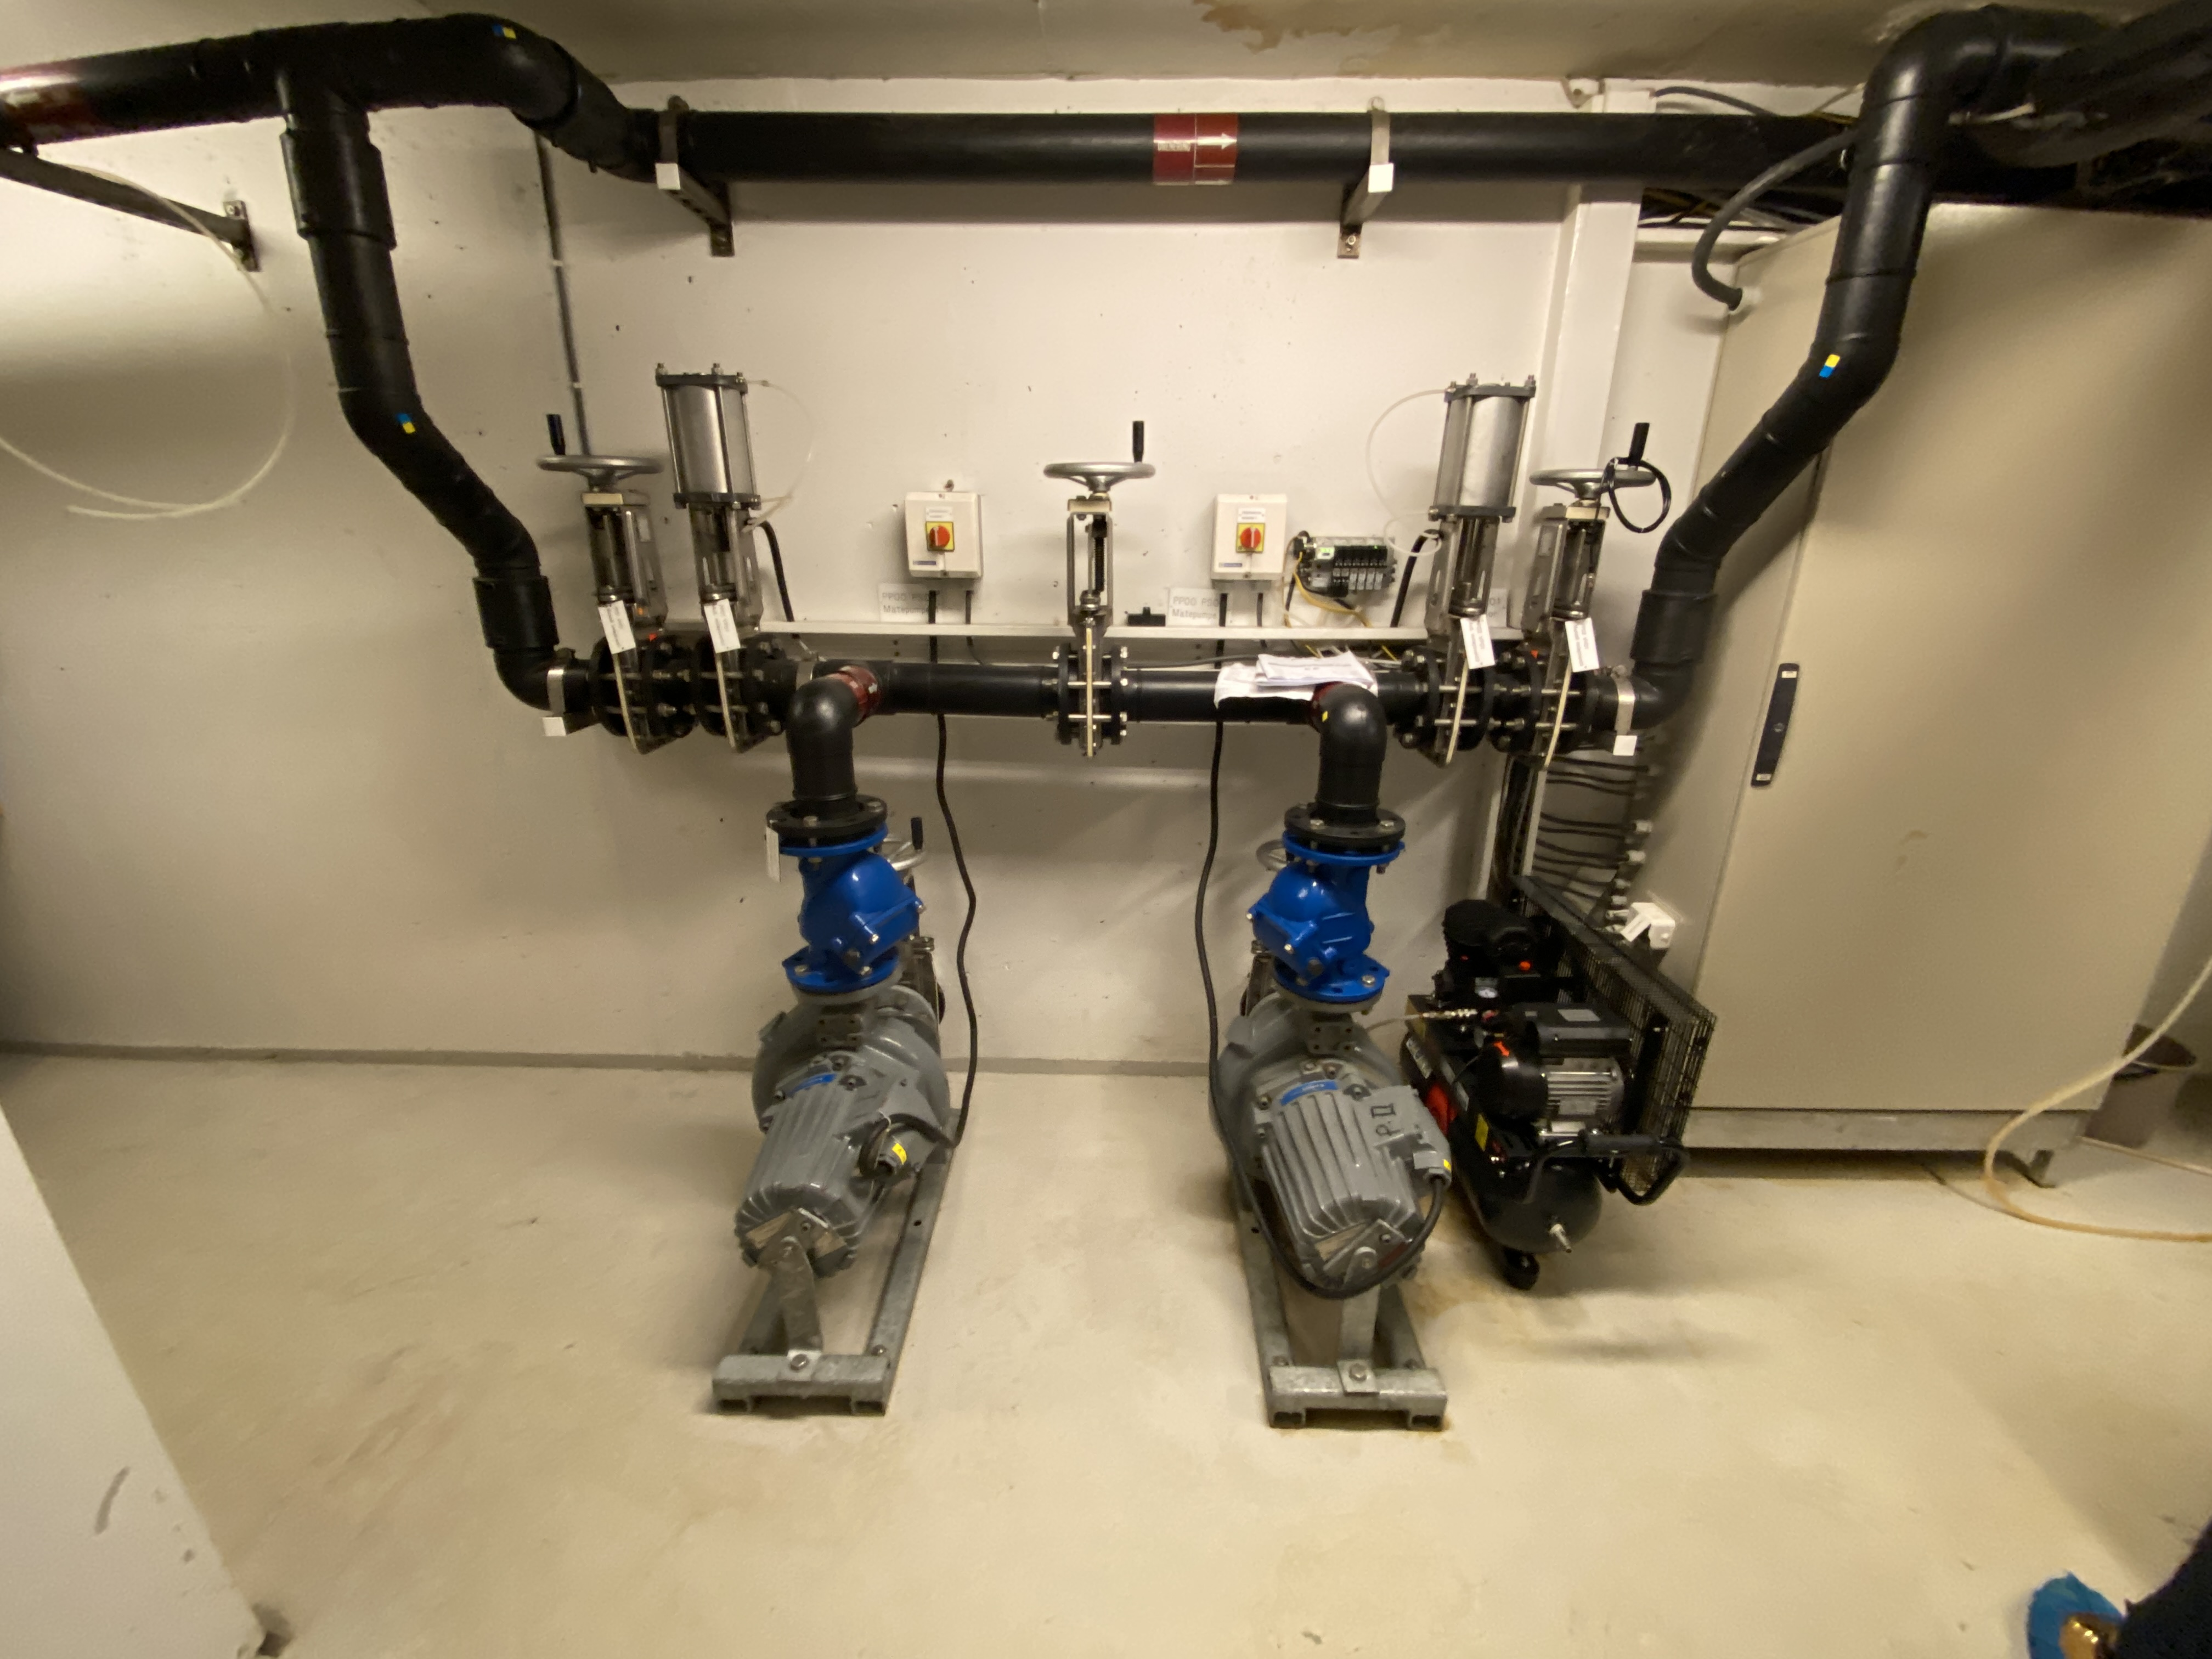
\includegraphics[width=1\textwidth]{Bilder/Bilde pumper.jpg}
    \caption{Matepumper}\label{fig:Matepumper}
\end{figure}

\newpage
\subsection{Reaktor}

Frå mottakstanken blir vatn pumpa opp mot reaktor dersom den er i riktig sekvens.
Vatn blir pumpa ved hjelp av to matepumper som rullerer, der kvar pumpe kan levere til kvar reaktor. 
Reaktorane er 165 $m^3$ og står på bakkenivå og strekker seg opp mot taket på bygget.
Reaktorane er utstyrt med nivåmåling via trykk og sensor er plassert to meter over botn.

I reaksjonssekvensen blir reaktorane periodisk lufta. Dette er for å lage aerobe og anaerobe fasar
for mikroorganismane som vidare gir betre reinsing.
For å best spreie oksygenet i den aerobe fasen
er det satt inn eit \gls{diffuser}-oppsett i botn.
\Gls{diffuser}ane er laga av ein membran med små hol som dannar bobler når lufta kjem i 
kontakt med avlaupsvatn.
Lufting av reaktoren gir også effektiv omrøring utan behov for ektra mekanisk inngrep.

\begin{figure}[htbp]
    \centering
    \begin{subfigure}[b]{0.3\textwidth}
        \centering
        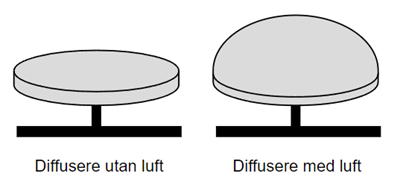
\includegraphics[width=1\textwidth]{Figurar/DiffusereMedOgUtanLuft.png}
        \caption{Illustrasjon \gls{diffuser}}\label{fig:Illustrasjon diffuser}
    \end{subfigure}
    \hfill
    \begin{subfigure}[b]{0.3\textwidth}
        \centering
        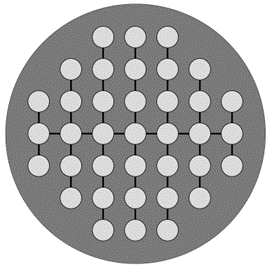
\includegraphics[width=1\textwidth]{Figurar/DiffuserFraTopp.png}
        \caption{Oppsett av \gls{diffuser}}\label{fig:Oppsett diffuser}
    \end{subfigure}
    \caption{\Gls{diffuser} system}\label{fig:Illustrasjon-Diffuser}
\end{figure}

På reinseanlegget er det tilleggskrav for fjerning av fosfor \citep{Regjeriga}. På grunn av desse tilleggskrava
er det sett inn eit tertiærreinsesteg ved hjelp av simultanfelling.
Simultanfelling er ein fellesbetegnelse på kombinert biologisk og kjemisk reinsing.

I slutten på reaksjonssekvensen tilsettest polyaluminium klorid, og kjemikaliet binder seg til
løyst fosfor og danner sedimenterbare partiklar \citep{Pax18}. Desse sedimenterbare partiklane synk 
så i sedimenteringssekvensen og utsleppskravet på fosfor oppretthaldast.

\begin{figure}[htbp]
    \centering
    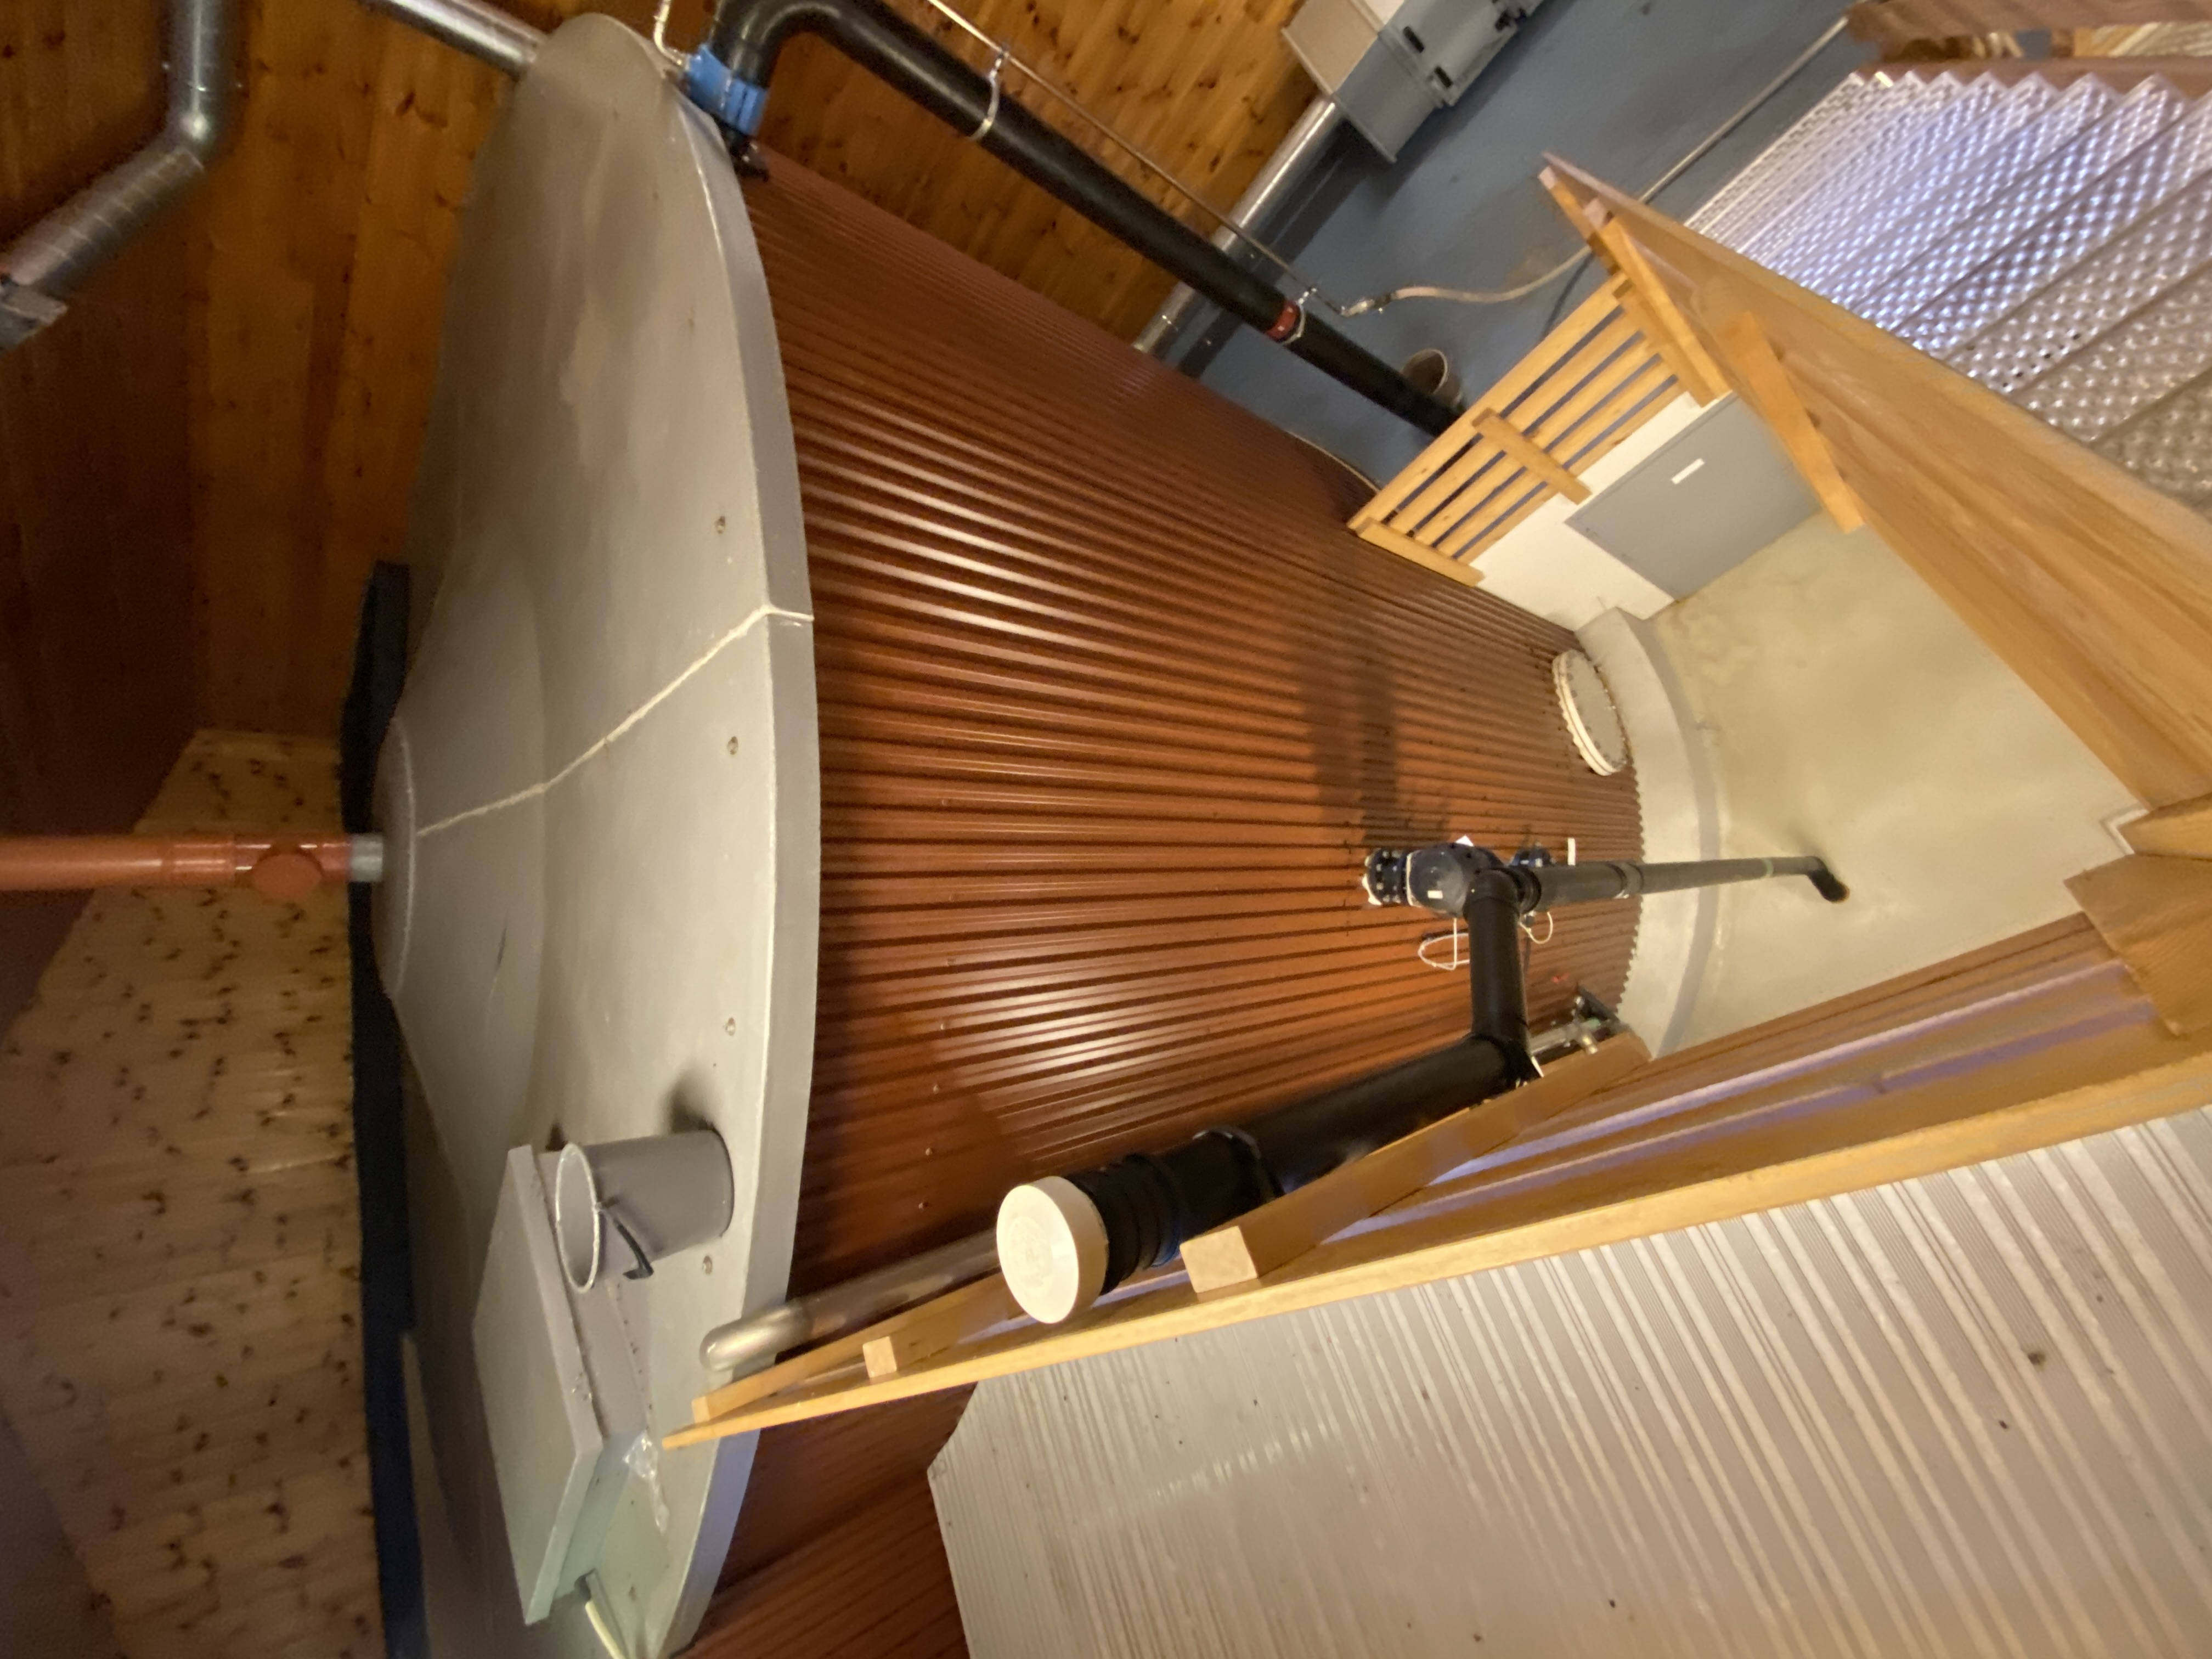
\includegraphics[angle=-90, width=1\textwidth]{Bilder/BildeReaktor.jpg}
    \caption{Reaktor}\label{fig:reaktorsoner}
\end{figure}

\newpage

Reaktorane er delt opp i tre forskjellige soner. Desse er med på å skilje
dei forskjellige substansane når reaktoren er ferdig med ein syklus.
Alle \gls{SBR}-reaktorar har lagra aktivert slam i botn \citep{Statsforvalter}. Det er her alle mikroorganismane akkumulerast 
og gir grunnlag for god biologisk reinsing. Denne sona blir kalla slamsona.\newline
Sjølve bruksvolumet til reaktoren er alt over uttaksventilen, 
og det er dette volumet som blir fylt og behandla under kvar innpumpingsekvens.

Mellom dei to sonene er det ei sikkerheitssone.
Denne sona er med for å ta hand om varierande sedimenteringseigenskapar
og eventuelt overskotsslam.\newline

\begin{figure}[htbp]
    \centering
    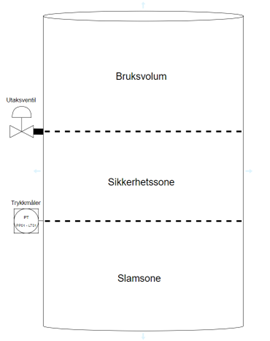
\includegraphics[width=0.5\textwidth]{Figurar/Reaktorsoner.png}
    \caption{Illustrasjon av reaktorsoner}\label{fig:Reaktorsonar}
\end{figure}

\subsection{P\&ID}

Det å setje seg inn i anleggets verkemåte skulle vise seg å være noko meir problematisk enn vi hadde forventa.
Hovudgrunnen til dette var at det ikkje fantest noko røyrgateskjema eller teknisk planteikning. \newline
Vi såg det som naudsynt å etablere ein \gls{PID} for å betre dokumentere og vise samanhengen til anlegget.

\begin{figure}[htbp]
    \centering
    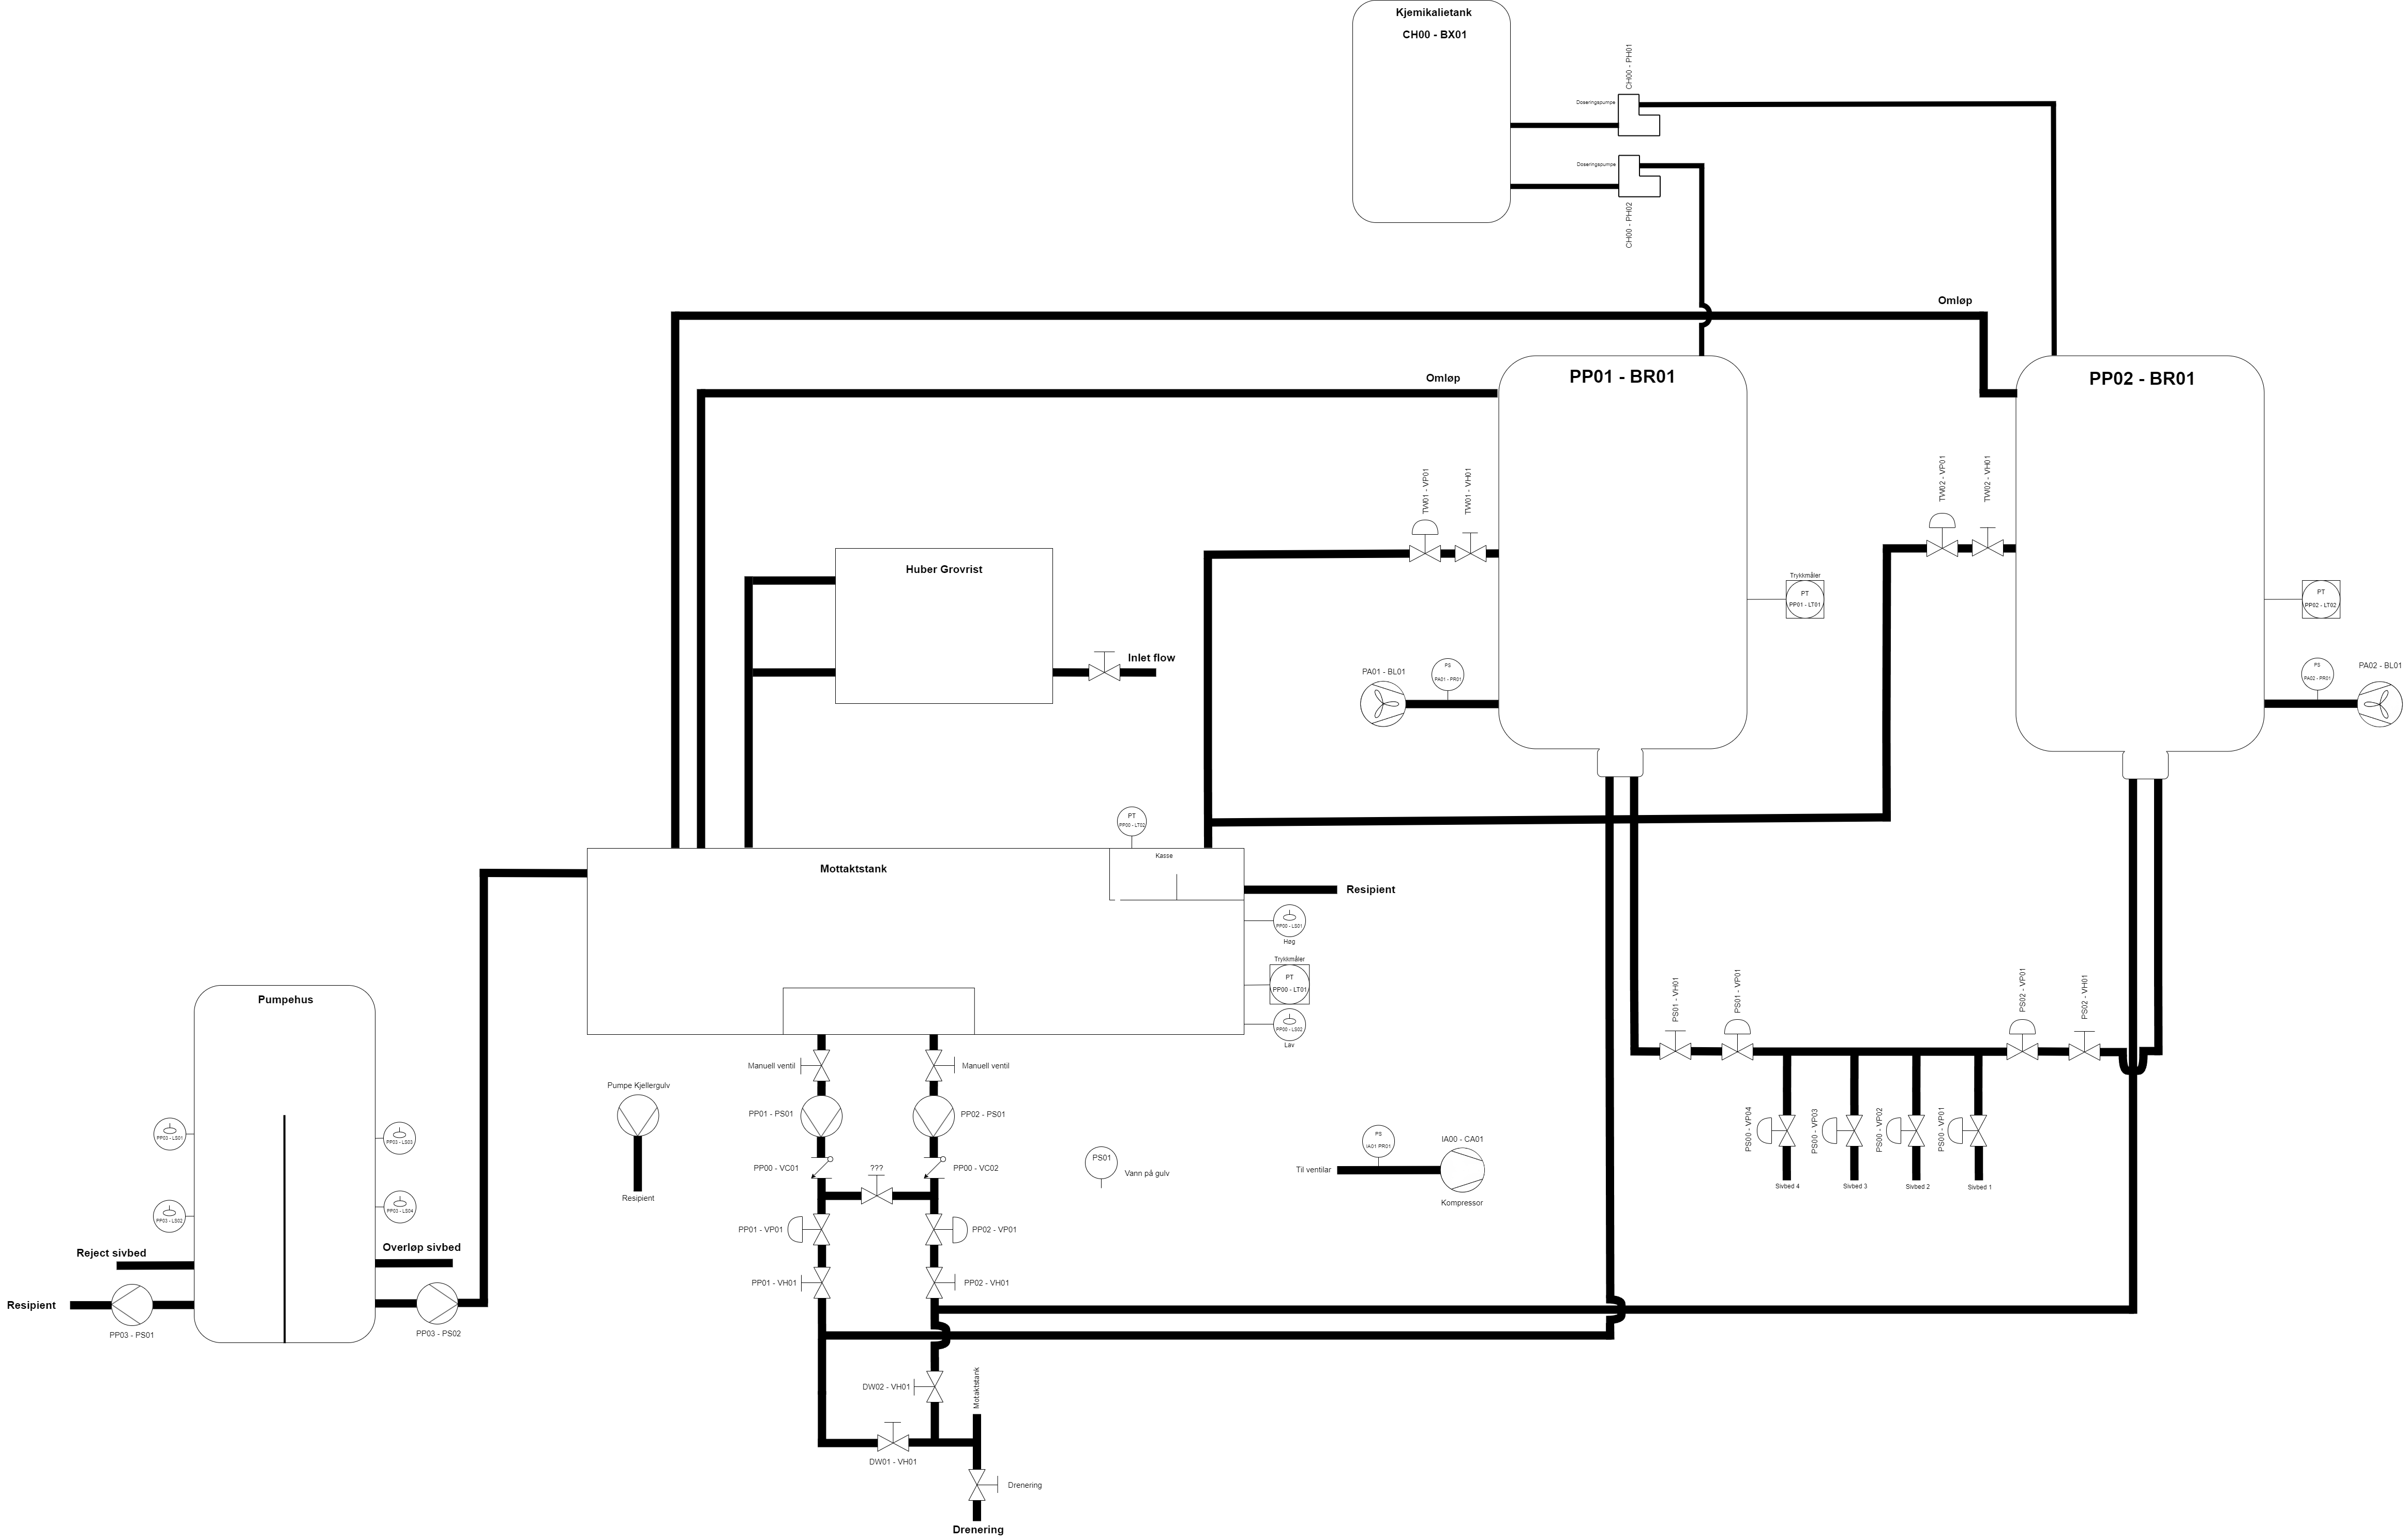
\includegraphics[angle=90,width=1\textwidth]{Figurar/PID.drawio.png}
    \caption{\gls{PID}}\label{fig:HMI}
\end{figure}